% !TEX TS-program = pdflatexmk

\documentclass{beamer}
\usepackage{times}
\usepackage{hyperref}
\usepackage{enumitem}

\mode<presentation>
{
  \usetheme{UAB}
  \setbeamercovered{transparent}
  \setbeamertemplate{headline}{}
  \setbeamertemplate{blocks}[rounded]
  \setbeamertemplate{navigation symbols}{}
}

\DeclareMathOperator*{\argmin}{argmin}
\DeclareMathOperator*{\argmax}{argmax}

\author{Steven Bethard}
\subject{CS 499: Senior Capstone}


\title{Anonymous 101}
\date{}

\begin{document}

\begin{frame}
\titlepage
\end{frame}

\begin{frame}{Quiz}
% "In Anonymous, hyperbolic manifestos and calls to apocalyptic action show you want to talk about an issue."
% Minimal police response to OpHBGary
% Anonymous vs. Sony: $31 -> $25 per share
% Lulzsec vs. Sony, Senate, CIA, FBI, Minecraft, Eve Online, Nintendo, etc. - unsophisticated hacks
% Lulzsec -> Antisec
% BART cut cell service; Anonymous take down BART websites, dump data
% Anonymous supports Occupy Wall Street
%
% How much does Anonymous matter?
%
% http://en.wikipedia.org/wiki/Timeline_of_events_associated_with_Anonymous
What is Anonymous's most heavily used attack method?
\begin{enumerate}[(A)]
\item<1-2> Distributed denial of service % Low orbit ion cannon (LOIC), High orbit ion cannon (HOIC)
\item<1> Ordering unpaid pizzas
\item<1> Exploiting weak passwords
\item<1> Protests and demonstrations
\item<1> SQL injection
\end{enumerate}
What was Anonymous's first attack against a major political player?
\begin{enumerate}[(A)]
\item<1> OpEgypt % Jan-Feb 2011, similar to OpTunisia; ended by Hosni Mubarak shutting off internet
\item<1> Project Chanology % 2008, against Scientology takedowns of Tom Cruise video
\item<1> OpTunisia % Jan 2011, "care package" to workaround Tunisian privacy restrictions
\item<1> Operation Avenge Assange % Dec 2010, against MasterCard, Visa, PayPal for freezing Assange's assets (attack against Amazon didn't work)
\item<1-2> Operation Payback is a b**** % Sep 2010, against MPAA, RIAA and AiPlex (which DDOSed the Pirate Bay)
\end{enumerate}
\end{frame}

\begin{frame}{Distributed Denial of Service Attacks}
\begin{center}
\href{http://www.youtube.com/watch?v=xR_lHN8wKHA\#t=2m3s}{\beamergotobutton{DDoS Attack Types}}
\end{center}
\visible<2->{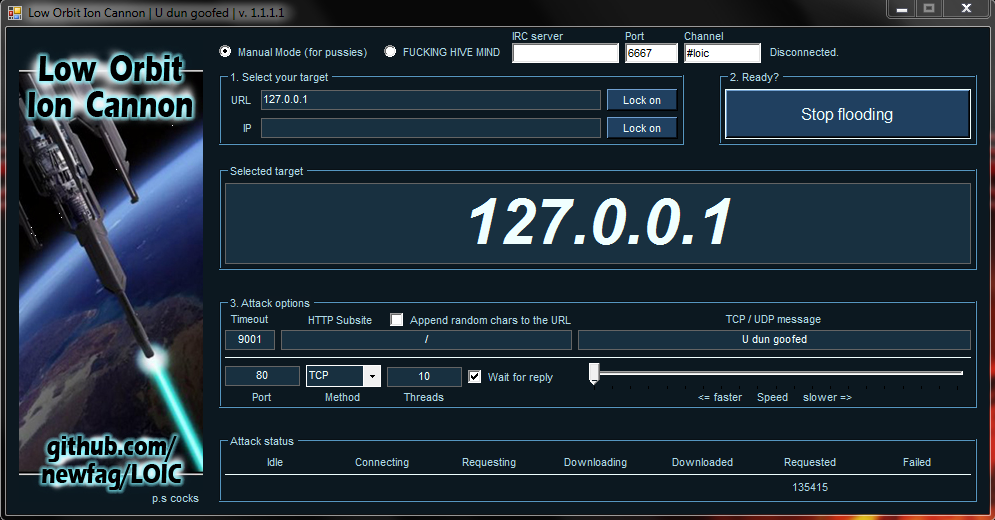
\includegraphics[width=\textwidth]{loic.png}}
\end{frame}

\begin{frame}{Other Attacks}
\begin{itemize}
\item \href{http://abclocal.go.com/kabc/story?id=6606733}{No Cussing Club, 2009}
% http://www.vcstar.com/news/2009/jan/15/teenage-founder-of-no-cussing-club-under-siege/
% for: "free speech"; by: pizzas, porno subscriptions, etc.
\item \href{http://www.thejournal.ie/fine-gael-website-defaced-by-anonymous-hacktivists-66151-Jan2011/}{Fine Gael, 2011}
% http://www.bbc.co.uk/news/uk-northern-ireland-12151724
% for: ?bad security?; by: comment field - JavaScript injection
\item \href{http://www.nytimes.com/2011/07/01/us/01orlando.html?_r=0}{Orlando, 2011}
% for: ability to feed homeless; by: DDoS
\item \href{http://www.zdnet.com/blog/security/anonymous-hacks-hundreds-of-chinese-government-sites/11303}{China, 2012}
%http://blogs.wsj.com/chinarealtime/2012/04/04/anonymous-hacks-chinese-government-websites/
%http://www.cnn.com/2012/04/06/world/asia/anonymous-china-hackers/
% for: restricting internet; by: ?admin passwords?
\item \href{http://www.zdnet.com/feds-stumbling-after-anonymous-launches-operation-last-resort-7000010541/}{US Sentencing Commission, 2013}
% http://www.businessinsider.com/anonymous-hacks-us-sentencing-commission-2013-1
% for: Aaron Schwartz; by: "injection apparatus"
\item \href{http://www.nbcnews.com/technology/anonymous-brandjacks-westboro-baptist-church-facebook-1C9395459}{Westboro Baptist Church, 2013}
% for: "god hates fags" stance; by: "brandjacking"
\end{itemize}
\bigskip
\pause
\begin{itemize}
\item What provoked the attack?
\item What form did the attack take?
\item What were the consequences?
\item Was the attack ethical? (Under which ethical code?)
\end{itemize}
\end{frame}

\begin{frame}{Not so Anonymous: Recently sentenced hackers}
\begin{itemize}
% http://www.nj.com/news/index.ssf/2009/11/verona_man_admits_hacking_chur.html
\item Dmitriy Guzner, 2009
\begin{description}
\item[Operation]: Project Chanology (DDoS) 2008
\item[Evidence]: username in Anonymous video
\item[Sentence]: 366 days in prison + 2 years of probation
\end{description}
% http://www.theguardian.com/technology/2013/jan/24/anonymous-hackers-jailed-cyber-attacks
% http://www.theregister.co.uk/2012/12/14/uk_anon_investigation/
\item Christopher Weatherhead, Ashley Rhodes, 2013
\begin{description}
\item[Operation]: Avenge Assange (DDoS) 2010
\item[Evidence]: IRC admin usernames $\Rightarrow$ ``open source research''
\item[Sentence]: 18 months in prison, 7 months in prison (UK)
\end{description}
% http://nakedsecurity.sophos.com/2013/09/15/anonymous-hacker-kahuna-sentenced-to-3-years-for-hacking-police-sites/
\item John Anthony Borell III, 2013
\begin{description}
\item[Operation]: OpPiggyBank (hacking of police sites) 2012
\item[Evidence]: tweets and IP address revealed by Twitter
\item[Sentence]: 3 years in prison
\end{description}
% http://www.theguardian.com/technology/2013/nov/15/jeremy-hammond-anonymous-hacker-sentenced
% http://www.theguardian.com/technology/2015/jan/22/barrett-brown-trial-warns-dangerous-precedent-hacking-sentencing
\item Jeremy Hammond, 2013 \visible<2->{(Barrett Brown, 2015, 5 years for linking)}
\begin{description}
\item[Operation]: Stratfor (hacking of security firm) 2011
\item[Evidence]: FBI informant Sabu in Lulzsec
\item[Sentence]: 10 years in prison
\end{description}
\end{itemize}
\end{frame}

\end{document}
